\documentclass{article}

\setlength{\textheight}{25.7cm}
\setlength{\textwidth}{16cm}
\setlength{\unitlength}{1mm}
\setlength{\topskip}{2.5truecm}
\topmargin 260mm \advance \topmargin -\textheight 
\divide \topmargin by 2 \advance \topmargin -1in 
\headheight 0pt \headsep 0pt \leftmargin 210mm \advance
\leftmargin -\textwidth 
\divide \leftmargin by 2 \advance \leftmargin -1in 
\oddsidemargin \leftmargin \evensidemargin \leftmargin
\parindent=0pt

\frenchspacing

\usepackage[english]{babel}
\usepackage{amsmath}
\usepackage{float}
\usepackage{graphicx}
\usepackage{subcaption}
\usepackage{tikz}
\usepackage{listings}

\pagestyle{empty}

\def\layersep{3.5cm}

\restylefloat{table}

\usepackage{listings}
\lstset{language=C++, showstringspaces=false, basicstyle=\small,
  numbers=left, numberstyle=\tiny, numberfirstline=false,
  stepnumber=1, tabsize=4, 
  commentstyle=\ttfamily, identifierstyle=\ttfamily,
  stringstyle=\itshape}

\title{Neural Networks: Assignment 2}
\author{Pepijn van Heiningen \\ \texttt{pvheinin@liacs.nl} \and Michiel Vos \\ \texttt{msvos@liacs.nl}}

\begin{document}

\maketitle

\section{Task 1: Function Optimization}
\subsection{Problem Description}
For the second assignment of Neural Networks we were given the task to optimize the Rosenbrock function using five different algorithms, and subsequently compare their performance, in order to get an insight into the advantages, disadvantages and limitations of the different algorithms.\\
\begin{figure}[H]
\[f(x,y) = 100 * (y-x^2)^2 + (1 - x)^2\]
\caption{The Rosenbrock's function}
\label{eq:rosen}
\end{figure}
The Rosenbrock function is a function that is used as a performance test for optimization algorithms. The equation can be found in figure \ref{eq:rosen}. It has a global minimum at the point (1,1), where the value of $f = 0$. This is visualized in figure \ref{fig:rosenbrock}. \\

\begin{figure}[H]
	\centering
		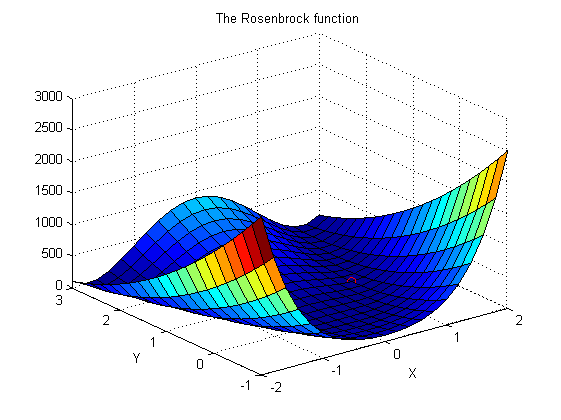
\includegraphics[scale=0.8]{rosenbrock.png}
	\caption{The Rosenbrock function, with minimal point}
	\label{fig:rosenbrock}
\end{figure}

\newpage
The 5 different algorithms we tested are:
\begin{itemize}
\item Gradient descent
\item Gradient descent with line search
\item Scaled conjugate gradient
\item Conjugate gradient
\item Quasi-Newton
\end{itemize}

To get a good comparison between the algorithms, each algorithm was run 100 times.
We first generated 100 random points around (-1,1) as starting points. Each algorithm was started from the same random point.\\

There were 4 different measures to compare the algorithms with:
\begin{itemize}
\item The average number of evaluations of $f$
\item The average number of evaluations of the gradient of $f$
\item The average run time of the algorithm
\item The average ``success rate''. 
\end{itemize}

Together these measures should provide a decent indication which algorithm performs better. Because some functions might be a lot more computationally expensive to evaluate than the Rosenbrock function, the number of evaluations of both the function and the gradient should be as low as possible. A run obviously shouldn't take too long, and it should have a high success rate. \\

The success rate is measured as reaching the minimum with an accuracy of 0.0001. This means that when the optimal point found by the algorithm is evaluated, the value of $f$ is smaller than 0.0001. Of course we would like to have an optimizer that gets a 100\% accuracy every time the algorithm is ran, but that is not always possible. 

\subsection{Implementation}
As described in the assignment, we run the algorithms using 100 randomly generated starting points from the distribution \texttt{[-1, 1] + 0.5 * randn(1,2)}. 

We set the options of the algorithm to the default options, with a few changes, we set the tolerance of the function value to $1*10^{-8}$, the iterations to 100, and we use a different learning rate for the two gradient descent algorithms. The reasoning behind the value is described in section \ref{sec:experiments}.
%Partial derivatives of f

In figure \ref{fig:partdiv}, we show the partial derivatives of the Rosenbrock function.
\begin{figure}[H]
    \[\frac{\partial f}{\partial x} = 400x^3 + 2x - 400*yx - 2\]
    \[\frac{\partial f}{\partial y} = 200y - 200*x^2\]
    \caption{Partial derivatives of $f$}
    \label{fig:partdiv}
\end{figure}

%\newpage
%In figure \ref{fig:pseudocode} you can see the pseudo-code of the implemented algorithm.

%\begin{figure}[H]
%\begin{verbatim}
%    starting_point = repmat([-1,1],100,1) + 0.5*randn(100,2);
%    options = foptions;         % Standard options
%    options(1) = -1;            % Turn off printing completely
%    options(3) = 1e-8;          % Tolerance in value of function
%    options(14) = 100;          % Max. 100 iterations of algorithm
%    options(18) = 0.001;        % Learning rate    
%    default_options = options;		
%    functionList = {@graddesc, @graddesc, @scg, @conjgrad, @quasinew};
%    for i = 1:100
%        for j = 1:5
%            options = default_options;
%            if(j==1 || j==2)
%                options(18) = 0.008;
%            end
%            if(j==2)
%                options(7) = 1;
%            end
%            tic;
%            [dump, options, dump, dump] = functionList{j}('rosen', starting_point(i,:),
%                                                                        options, 'rosegrad');
%            time = toc;
%            results(i,j,1) = options(10);
%            results(i,j,2) = options(11);
%            results(i,j,3) = time;
%            results(i,j,4) = options(8);
%        end 
%    end  
%\end{verbatim}
%\caption{Pseudo-code of task 1.}
%\label{fig:pseudocode}
%\end{figure}

\newpage
\subsection{Experiments}
\label{sec:experiments}
%Gradient descent experiments
In task $1.3$ we were asked to tune both gradient descent algorithms manually. We first kept the number of iterations to 100, and tested different values of the learing rate. The results are in table \ref{tab:learningrate}.

\begin{table}[H]
    \parbox{.45\linewidth}{
	\centering
		\begin{tabular}{|l|l|l|l|}
        \hline
		Iterations & Learning rate & GD & GD /w linesearch \\ \hline 
		100 & 0.05 & 0 \% & 5.4 \% \\ \hline
		100 & 0.01 & 0 \% & 5.8 \% \\ \hline
		100 & 0.008 & 0 \% & 5.8 \% \\ \hline
		100 & 0.005 & 0 \% & 5.6 \% \\ \hline
		100 & 0.001 & 0 \% & 3.8 \% \\ \hline
		\end{tabular}
    }
    \hfill
    \parbox{.45\linewidth}{
	\centering
		\begin{tabular}{|l|l|l|l|}
        \hline
		Iterations & Learning rate & GD & GD /w linesearch \\ \hline 
		100.000 & 0.008 & 0 \% & 100 \% \\ \hline
		\end{tabular}
    }
    \caption{Optimizing the learning rate}
    \label{tab:learningrate}
\end{table}
    
The values are averages over 500 runs. We then tested the best value on 100 runs with 100.000 iterations, and the gradient descent algorithm with line search reached an accuracy of 100\%. The standard gradient descent still got 0\%.
As you can see the optimal error for gradient with line search is somewhere around a learning rate of 0.008, which is why we set the learning rate for the experiment to that value. To find out why the normal gradient descent does not produce any results, we plotted the search paths. There we can see that the learning rate is probably too high for normal gradient descent, which is why it diverges. \\

\begin{figure}[H]
	\centering
	\begin{subfigure}[b]{0.45\textwidth}
		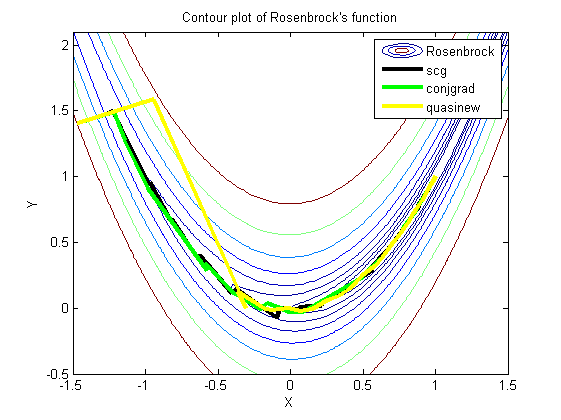
\includegraphics[width=\textwidth]{rosenbrocktask1.png}
		\label{fig:rosenbrocktask1.1}
	\end{subfigure}
	\begin{subfigure}[b]{0.45\textwidth}
		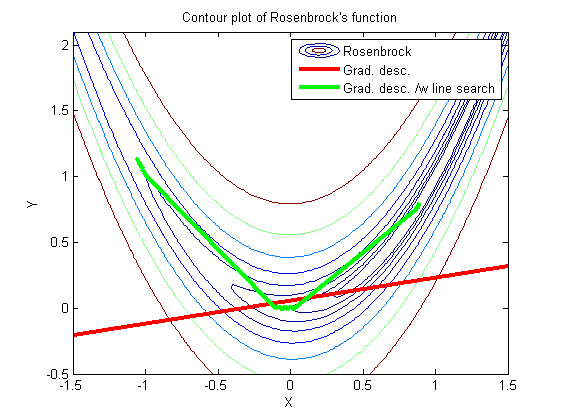
\includegraphics[width=\textwidth]{rosenbrocktask12.png}
		\label{fig:rosenbrocktask1.2}
	\end{subfigure}	
	\caption{Search paths of different functions}
\end{figure}

\begin{table}[H]
	\centering
	\begin{tabular}{| l | l | l | l | l |}
		\hline
		Function                        & Evaluation  & Gradient evaluation & Runtime & Successrate \\ \hline 
		Gradient descent                & 101         & 100  & 0.003          & 0\% \\ \hline
		Gradient descent /w line search & 1836.4      & 98.8   & 0.090          & 4\% \\ \hline
		Scaled conjugate gradient       & 45.38        & 69.64  & 0.002  & 100\% \\ \hline
		Conjugate gradients             & 274.15        & 18.09 & 0.014        & 100\% \\ \hline
		Quasi-Newton                    & 92.39        & 27.41 & 0.006  & 100\% \\ \hline
	\end{tabular}
	\caption{Results of the 5 algorithms. All values are averages.}
	\label{tab:results}
\end{table}

In table \ref{tab:results} you can find the results of the different algorithms. All 5 algorithms were run on an Intel Core i5-3470, the values are averages over 100 runs. 
%The parameters used for the algorithms are described in the section `Implementation'.
The amount of maximum iterations are set to 100 and the learning rate is set to 0.001.
As you can see the gradient descent algorithm, even after optimization, still achieves a success rate of 0\% on the data. If we look at the output-coordinates of the algorithm, it shows that this setting of the learning rate is too high, because the coordinates keep growing until they reach infinity. Gradient descent with line search already works a lot better, but it costs more function evaluations. The other three methods clearly achieve better results on all measured objectives, with less evaluations, a shorter runtime and higher success rates.

\subsection{Conclusions}
%Which algorithm is best? Which is worst?
%What is the expected number of function evaluations (including evaluations of gradients)
%needed to reach the optimum? What might be the reason for the very poor performance
%of the gradient descent algorithm?
It is difficult to select the best algorithm. Both the Scaled Conjugate Gradient approach and the Quasi-Newton algorithm perform well on this particular problem. The Scaled Conjugate Gradient uses less function evaluations than Quasi-Newton, but Quasi-Newton uses less gradient evaluations. The runtime of both algorithms is almost equal, and they both achieve a success rate of 100\%. It will depend on the computational difficulty of the problem to determine which algorithms is better. \\\\
The worst algorithm is clearly gradient descent, since it doesn't find good solutions, even in 100 runs there are no successful solutions. This can also be because the learning rate is not set optimally. Gradient descent with line search is the slowest algorithm of them all, but because it does produce some useful solutions it is better than the original gradient descent algorithm.
The reason for the very poor performance of the gradient descent algorithm is probably that if the learning rate is set too high, the algorithms best coordinates will `explode' into infinity. If the learning rate is set to a lower rate, 100 iterations are not enough to get to the optimal point. Because the Rosenberg function has such a narrow valley, finding the optimal value is very difficult.

\newpage
\section{Task 2}
\subsection{Problem Description}
Instead of trying to find the minimum of the Rosenbrock's function in task 1, we were asked to solve the "exclusive or" (xor) problem in task 2. Given two bits, the correct output bit should be returned. Please see table~\ref{tab:tt} for the truth table.

\begin{table}[H]
	\centering
	\begin{tabular}{| l | c | r |}
		\hline
		$x_1$ & $x_2$ & $y$ \\ \hline
		0 & 0 & 0 \\ \hline
		0 & 1 & 1 \\ \hline
		1 & 0 & 1 \\ \hline
		1 & 1 & 0 \\ \hline
	\end{tabular}
	\caption{The truth table. When only one of the two input bits is true, the output bit should be true.}
	\label{tab:tt}
\end{table}

A perceptron cannot solve this problem, because the classes (different values of y) could not be separated linearly with one line in twodimensional space. This is shown if figure \ref{fig:sep}.

\begin{figure}[H]
	\centering
	\begin{subfigure}[b]{0.3\textwidth}
		\begin{tikzpicture}[x=1cm,y=1cm]
			\draw[latex-latex, thin, draw=gray, ->] (0,0)--(2,0) node [right] {$x_1$};
			\draw[latex-latex, thin, draw=gray, ->] (0,0)--(0,2) node [above] {$x_2$}; 
			\draw[thick] (-1, -0.5)--(1.5, 2); 

			\draw [dotted, gray] (-1, -1) grid (2, 2);
			\node [black] at (0, 1) {\textbullet};
			\node [black] at (-0.2, 1) {$_1$};
			\node [black] at (1, 0) {\textbullet};
			\node [black] at (1, -0.2) {$_1$};
			\node [black] at (0, 0) {$\circ$} node [below left] {$_0$};
			\node [black] at (1, 1) {$\circ$};
		\end{tikzpicture}
		\caption{}
	\end{subfigure}
	\begin{subfigure}[b]{0.3\textwidth}
		\begin{tikzpicture}[x=1cm,y=1cm]
			\draw[latex-latex, thin, draw=gray, ->] (0,0)--(2,0) node [right] {$x_1$};
			\draw[latex-latex, thin, draw=gray, ->] (0,0)--(0,2) node [above] {$x_2$}; 
			\draw[thick] (-0.5,-1)--(2, 1.5);

			\draw [dotted, gray] (-1, -1) grid (2, 2);
			\node [black] at (0, 1) {\textbullet};
			\node [black] at (-0.2, 1) {$_1$};
			\node [black] at (1, 0) {\textbullet};
			\node [black] at (1, -0.2) {$_1$};
			\node [black] at (0, 0) {$\circ$} node [below left] {$_0$};
			\node [black] at (1, 1) {$\circ$};
		\end{tikzpicture}
		\caption{}
	\end{subfigure}
	\begin{subfigure}[b]{0.3\textwidth}
		\begin{tikzpicture}[x=1cm,y=1cm]
			\draw[latex-latex, thin, draw=gray, ->] (0,0)--(2,0) node [right] {$x_1$};
			\draw[latex-latex, thin, draw=gray, ->] (0,0)--(0,2) node [above] {$x_2$}; 
			\draw[thick] (-1, -0.5)--(1.5, 2); 
			\draw[thick] (-0.5,-1)--(2, 1.5);

			\draw [dotted, gray] (-1, -1) grid (2, 2);
			\node [black] at (0, 1) {\textbullet};
			\node [black] at (-0.2, 1) {$_1$};
			\node [black] at (1, 0) {\textbullet};
			\node [black] at (1, -0.2) {$_1$};
			\node [black] at (0, 0) {$\circ$} node [below left] {$_0$};
			\node [black] at (1, 1) {$\circ$};
		\end{tikzpicture}
		\caption{}
	\end{subfigure}
	\caption{3 trials to separate the classes. The filled circles are true cases and the empty circles are false cases.}
	\label{fig:sep}
\end{figure}

As seen in figure~\ref{fig:sep} (c) it is possible to solve the xor problem, but not with a perceptron. We need something more advanced, like a neural network with a hidden layer.


 
\begin{figure}[H]
    \centering
	\begin{tikzpicture}[shorten >=1pt,->,draw=black!50, node distance=\layersep]
	   	\tikzstyle{every pin edge}=[<-,shorten <=1pt]
		\tikzstyle{neuron}=[circle,fill=black!25,minimum size=17pt,inner sep=0pt]
		\tikzstyle{input neuron}=[neuron, fill=green!50];
		\tikzstyle{output neuron}=[neuron, fill=red!50];
	   	\tikzstyle{hidden neuron}=[neuron, fill=blue!50];
		\tikzstyle{annot} = [text width=4em, text centered]

		% Draw the input layer nodes
		\node[input neuron, pin=left:$x_1$] (I-1) at (0,-1) {};
		\node[input neuron, pin=left:$x_2$] (I-2) at (0,-3) {};

		\path node[hidden neuron] (H-1) at (\layersep,-1 cm) {};
		\path node[hidden neuron] (H-2) at (\layersep,-3 cm) {};

	    	% Draw the output layer node %[yshift=0.5cm]
	    	\node[output neuron,pin={[pin edge={->}]right:$y = \varphi(net) = \varphi(y_1u_1 + y_2u_2)$}, right of=H-1, yshift=-1.0cm] (O) {};

		% Connect every node in the input layer with every node in the
		% hidden layer.
		\path (I-1) edge node [above] {$w1$} (H-1) ;
		\path (I-1) edge node [pos=0.75, below, sloped] {$w3$} (H-2);
		\path (I-2) edge node [pos=0.75, above, sloped] {$w2$} (H-1);
		\path (I-2) edge node [below] {$w4$} (H-2);

		% Connect every node in the hidden layer with the output layer
		\path (H-1) edge node [above, sloped] {$w5$} (O);
		\path (H-2) edge node [below, sloped] {$w6$} (O);

		% Annotate the layers
		\node[annot,above of=H-1, node distance=1cm] (hl) {Hidden layer};
		\node[annot,left of=hl] {Input layer};
		\node[annot,right of=hl] {Output layer};
	\end{tikzpicture}
	\caption{Visualitation of the xor net.}
	\label{fig:nn}
\end{figure}

\newpage
\subsection{Solution}
We made a multilayer neural network with three nodes and six weights \footnote{The network could be trained much faster when bias nodes are used, but in sight of the assignment there is chosen to do it the hard way and make the problem more difficult.}. Please see Figure~\ref{fig:nn} for an illustration. The network is trained with the data of the truth table and the weights are updated with the algorithms of task 1. The algorithm tries to steer the weights in such a way the errors of the predicted classes and the actual classes are minimized.

\subsection{Implementation}
\begin{figure}[H]
	\centering
	\begin{eqnarray}
		net_1 &&= w_1x_1 + w_2x_2 \\
		y_1 &&= \varphi(net_1) \\
		net_2 &&= w_3x_1 + w_4x_2 \\
		y_2 &&= \varphi(net_2) \\
		net &&= w_5y_1 + w_6y_2\\
		y &&= \varphi(net)
	\end{eqnarray}
	\caption{The computation of the output value, based on the input values and the weights.}
	\label{fig:net}
\end{figure}
%\begin{figure}[H]
%	\begin{lstlisting}[caption={The computation of the output value, based on the input values and the weights.}, captionpos=b, language=matlab, numbers=left, tabsize=4, frame=single, basicstyle=\footnotesize]
%	function [y] = xornet(x1, x2, w)
%		net1 = w(1) * x1 + w(2) * x2;
%	 	y1 = phi(net1);
%		net2 = w(3) * x1 + w(4) * x2;
%	 	y2 = phi(net2);
%		net = w(5) * y1 + w(6) * y2;
%	 	y = phi(net);
%	end
%	\end{lstlisting}
%\end{figure}

\begin{figure}[H]
	\centering
	\begin{eqnarray}
	 \varphi(x) & = & \frac{1}{1 + e^{-x}} \\
	   \varphi'(x) & = & \varphi(x)(1 - \varphi(x))
	\end{eqnarray}
	\caption{The sigmoid function (1) and the derivative (2).}
	\label{fig:sig}
\end{figure}

Figure~\ref{fig:net} computes the output value. The ($\varphi$) sigmoid (Figure~\ref{fig:sig}) is used as the activation function, so the output value will always lay between 0 and 1. The sum squared errors of the network are calculated with the formulas from Figure~\ref{fig:sse}. For every scenario of input values (all four combinations of $x_1$ and $x_2$) the computed value is subtracted with the actual value (which is found in the truth table). These values are squared and cumulated. The lower the result the better. Figure~\ref{fig:dsse} calculates the derivatives, which are used by the 5 algorithms. In order to check the correctness of the function we used the gradchek function of the Netlab toolbox. The results are in table~\ref{table:gradchek}. The values of the analytic column are computed with the formulas from Figure~\ref{fig:sse} and Figure~\ref{fig:dsse}. The values of the diffs column are approximated with a central difference formula with a very small step size. The deltas are the difference between the two methods and are very near to 0. The reason for this is because the gradcheck function produces an approximation. 




\begin{figure}[H]
	\centering
	\begin{eqnarray}
		E(w) = && (net(0, 0, w) - 0)^2 + \\
				&& (net(0, 1, w) - 1)^2 + \\
				&& (net(1, 0, w) - 1)^2 + \\
				&& (net(1, 1, w) - 0)^2
	\end{eqnarray}
	\caption{The calculation of the sum squared error of the weights.}
	\label{fig:sse}
\end{figure}
%\begin{figure}[H]
%	\begin{lstlisting}[caption={The calculation of the sum squared error of the weights.}, label={listing:mysse}, captionpos=b, language=matlab, numbers=left, tabsize=4, frame=single, basicstyle=\footnotesize, breaklines=true]
%function [d] = mysse(w)
%	d = power(xornet(0, 0, w) - 0, 2) + 
%		power(xornet(0, 1, w) - 1, 2) + 
%		power(xornet(1, 0, w) - 1, 2) + 
%		power(xornet(1, 1, w) - 0, 2);
%end
%	\end{lstlisting}
%\end{figure}

\begin{figure}[H]
	\centering
	\begin{eqnarray}
		\frac{\partial E}{\partial w_1} &&= \Sigma{(y - d)\varphi'(net)w_5\varphi'(net_1)x_1} \\
		\frac{\partial E}{\partial w_2} &&= \Sigma{(y - d)\varphi'(net)w_5\varphi'(net_1)x_2} \\
		\frac{\partial E}{\partial w_3} &&= \Sigma{(y - d)\varphi'(net)w_6\varphi'(net_2)x_1} \\
		\frac{\partial E}{\partial w_4} &&= \Sigma{(y - d)\varphi'(net)w_6\varphi'(net_2)x_2} \\
		\frac{\partial E}{\partial w_5} &&= \Sigma{(y - d)\varphi'(net)y_1} \\
		\frac{\partial E}{\partial w_6} &&= \Sigma{(y - d)\varphi'(net)y_2}
	\end{eqnarray}
	\caption{Cumulated partial derivatives of the sum squared error.}
	\label{fig:dsse}
\end{figure}



%\begin{figure}
%	\begin{lstlisting}[caption={The computation of the derivatives of the sum squared error of the weights.}, label={listing:dmysse}, captionpos=b, language=matlab, numbers=left, tabsize=4, frame=single, basicstyle=\footnotesize, breaklines=true, deletekeywords={input, zeros}]
%function [d] = dmysse(w)
%	d = zeros(1, 6);

%	input = [0, 0; 0, 1; 1, 0; 1, 1];
%	target = [0, 1, 1, 0];

%	for i = 1:4
%		net1 = w(1) * input(i, 1) + w(2) * input(i, 2);
%		y1 = phi(net1);
%		net2 = w(3) * input(i, 1) + w(4) * input(i, 2);
%		y2 = phi(net2);
%		net = w(5) * y1 + w(6) * y2; 
%		y = phi(net);
	
%		d(1) = d(1) + (y - target(i)) * phiprime(net) * w(5) * phiprime(net1) * input(i, 1);
%		d(2) = d(2) + (y - target(i)) * phiprime(net) * w(5) * phiprime(net1) * input(i, 2);
%		d(3) = d(3) + (y - target(i)) * phiprime(net) * w(6) * phiprime(net2) * input(i, 1);
%		d(4) = d(4) + (y - target(i)) * phiprime(net) * w(6) * phiprime(net2) * input(i, 2);
%		d(5) = d(5) + (y - target(i)) * phiprime(net) * y1;
%		d(6) = d(6) + (y - target(i)) * phiprime(net) * y2;
%	end
%	d = d * 2;
%end
%	\end{lstlisting}
%\end{figure}

\begin{table}[H]
	\centering
	\begin{tabular}{| l | l | l | l |}
		\hline
		Weight & Analytic & Diffs & Delta \\ \hline
$w_1$ & -0.0050 & -0.0050 & $5.4682*10^{-11}$ \\ \hline
$w_2$ & -0.0032 & -0.0032 & $1.1398*10^{-10}$ \\ \hline
$w_3$ & 0.06435 & 0.06435 & $-1.8951*10^{-11}$ \\ \hline
$w_4$ & 0.04339 & 0.04339 & $-3.2260*10^{-11}$ \\ \hline
$w_5$ & 0.18566 & 0.18566 & $6.0969*10^{-11}$ \\ \hline
$w_6$ & 0.18131 & 0.18131 & $1.0486*10^{-10}$ \\ \hline
	\end{tabular}
	\caption{Results of the gradchek function.}
	\label{table:gradchek}
\end{table}

\subsection{Experiments}
We ran all 5 algorithms for 100 iterations, starting from a random point. This is done 100 times to get the averages of the function evaluations, gradient evaluation and the success rate. The relative amount of times an algorithm is successful after 100 iterations is the success rate. An algorithm is succesful when it can predict all four scenarios correctly. The succcess rule is defined in Figure~\ref{fig:sr}. The results are in Table~\ref{table:results}. 


\begin{figure}[H]
	\centering
	\begin{eqnarray}
		success =&& round(net(0, 0, w)) == 0 \wedge \\
				&& round(net(0, 1, w)) == 1 \wedge \\
				&& round(net(1, 0, w)) == 1 \wedge \\
			&& round(net(1, 1, w)) == 0
	\end{eqnarray}
	\caption{Success rule}
	\label{fig:sr}
\end{figure}


%\begin{figure}[H]
%	\begin{lstlisting}[caption={Success condition of a set of weights.}, label={eq:success}, captionpos=b, language=matlab, numbers=left, tabsize=4, frame=single, basicstyle=\footnotesize, breaklines=true, deletekeywords={round}]
%success = 	round(xornet(0, 0, w)) == 0 & ...
%			round(xornet(1, 1, w)) == 0 & ... 
%			round(xornet(0, 1, w)) == 1 & ...
%			round(xornet(1, 0, w)) == 1;
%	\end{lstlisting}
%\end{figure}

%\newpage
\begin{table}[H]
	\centering
	\begin{tabular}{| l | l | l | l | l |}
		\hline
		Function & Evaluation & Gradient evaluation & Runtime (sec) & Successrate \\ \hline
		Gradient descent & 101 & 100 & 2.4 & 0\% \\ \hline
		Gradient descent (line search) & 1682 & 100 & 6.3 & 0\% \\ \hline
		Scaled conjugate gradient & 71 & 128 & 3.0 & 0\% \\ \hline
		Conjugate gradients & 1808 & 76 & 6.1 & 14\% \\ \hline
		Quasi-Newton & 249 & 85 & 2.5 & 16\% \\ \hline
	\end{tabular}
	\caption{Results of the 5 algorithms. All values are averages and rounded.}
	\label{table:results}
\end{table}

Another experiment was to see how well an naive produce will perform. We generated 10 million random weights sets and tested how many of the sets were successful. Only 8 were successful. 

\subsection{Conclusion}
Neural networks can solve the xor problem. The update function of the weights are important, because they have different performances. The success rate of the Quasi-Newton method is the highest, but how important is the success rate? We only need one solution to solve the problem and one successful set of weights is not better compared to another successful set of weigths. Gradient descent and scaled conjugate cannot solve this problem within the chosen boundaries. The naive approach of generating random solutions can solve the problem, it only takes a while. Note, probably all functions will perform better if we used bias nodes in the neural network.

\newpage
\section{Task 3: Handwritten Digit Recognition with MLP}
In task 3 we had to compare the Multilayer Perceptron networks to the single layer networks we have investigated in Assignment 1.

\subsection{Problem Description}
We were given the handwritten digits dataset from Assignment 1 again, and were now asked to implement a multilayer perceptron network, and train it to recognize handwritten digits.
The goal is of course to achieve the highest classification rate posssible.

\subsection{Implementation}
%Pseudocode
We built a Multi-Level perceptron with 256 inputs and 10 outputs. The inputs are the images and the outputs are the labels. Each output can be seen as a boolean value that is true if the input was the corresponding digit. 

%\begin{figure}[H]
%    \begin{verbatim}        
%    function task_3()
%        %Create the net
%        net = mlp(256,75,10,func);
%        %Train the nets
%        net = mlptrain(net, training', target_training, 100);
%        %Test errors on training
%        output_training = mlpfwd(net, training');
%        %Test errors on testset
%        output_test = mlpfwd(net, testdata');
%        %create confusion matrix for training
%        %create confusion matrix for testset
%    end
%    \end{verbatim}
%    \caption{Pseudo-code of task 1.}
%    \label{fig:code}
%\end{figure}

%\newpage
\subsection{Experiments}
We first tried to find the best number of hidden nodes. We set the number of training iterations to 100, and used the Scaled Conjugate Gradient as a training method. In the plot of figure \ref{fig:hidden_nodes} you can see that the softmax activation function yields the best results.

\begin{figure}[H]
	\centering
		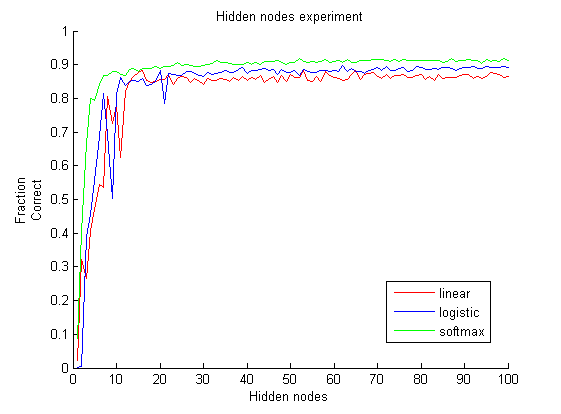
\includegraphics[scale=0.8]{hidden_nodes.png}
    \caption{Hidden nodes}
    \label{fig:hidden_nodes}
\end{figure}

Because there is no improvement after about 30 hidden nodes, we set the number of nodes to 75. To check whether there are differences between the Scaled Conjugate Gradient method, Quasi-Newton and Backpropagation, we show the classification rates and runtime in table \ref{tab:tm}.

\begin{table}[H]
	\centering
	\begin{tabular}{| l | l | l |}
		\hline
		Training method & Runtime & Classification rate \\ \hline
		SCG & 2.3550 & 93.84 \\ \hline
		Conjugate Gradient & 7.2546 & 93.42\\ \hline
		Backpropagation & 1.1860 & 65.74 \\ \hline
	\end{tabular}
	\caption{Comparison of training methods}
	\label{tab:tm}
\end{table}

The values are averages over 20 runs. Quasi-Newton was not tested, because it used too much RAM for our pc (which has 8GB). 

%\newpage
Finally we tried to find the best value for the number of training iterations. (See table \ref{tab:trainiter})
\begin{table}[H]
	\centering
	\begin{tabular}{| l | l | l |}
		\hline
		Training iterations & Runtime & Average classification rate \\ \hline

            1 &   0.0567  &  27.62 \\ \hline
           11 &   0.2825  & 90.31 \\ \hline
           21 &   0.4920  & 92.56 \\ \hline

           31 &   0.6624  & 93.73\\ \hline
           41 &   0.8748  & 93.48 \\ \hline
           51 &   1.0392  & 93.82 \\ \hline

           61 &   1.2038  & 93.84 \\ \hline
           71 &   1.3936  & 93.81 \\ \hline
           81 &   1.6338  & 94.12 \\ \hline
           91 &   1.7814  & 93.79 \\ \hline
	\end{tabular}
	\caption{Comparison of training iterations, averaged over 10 runs.}
	\label{tab:trainiter}
\end{table}

As we expected there is a minimum of training iterations necessary to train the network properly, but after that threshold is reached, no more improvement is found. This is why we set the training iterations to 50.

\subsubsection{Activation functions}
In figure \ref{fig:errormeasure} you can see the different functions and the way their error values are calculated.

\begin{figure}[H]
	\centering
%	edata = 0.5*sum(sum((y - t).^2));
	\begin{eqnarray}
		&& \frac{1}{2}(y - t)^2 \\
		&&-(t * log(y) + (1 - t) * log(1 - y)) \\
		&& -t * log(y)
	\end{eqnarray}
	\caption{Error measurements in multiple activation functions. (1) Linear (2) Logistic (3) Softmax }
    \label{fig:errormeasure}
\end{figure}

\subsection{Conclusions}
The final algorithm used a network with 75 hidden nodes, 50 training iterations and the Scaled Conjugate Gradient method for training the network. Finally we ran the algorithm 100 times, mixing up the test and trainingset each run, checking the algorithm only on input digits that it hasn't seen before. We achieved a final accuracy of $93.72\%$.



\end{document}
